\documentclass{article}
\usepackage[utf8]{inputenc}
\usepackage{amsfonts}
\usepackage{listings}
\usepackage{xcolor}
% Using the absolute value!
\usepackage{mathtools}
\usepackage{graphicx}
\usepackage{enumitem}
\usepackage{cite}
\DeclarePairedDelimiter\abs{\lvert}{\rvert}
\usepackage{vmargin}
\makeatletter
\let\oldabs\abs
\def\abs{\@ifstar{\oldabs}{\oldabs*}}
\usepackage{neuralnetwork}
% MARGINS
\setpapersize{A4}
\setmargins{2.5cm}       
{1.5cm}                        
{16.5cm}                      
{23.42cm}                   
{10pt}                           
{1cm}                           
{0pt}                             
{2cm}                           
\definecolor{codegreen}{rgb}{0,0.6,0}
\definecolor{codegray}{rgb}{0.5,0.5,0.5}
\definecolor{codepurple}{rgb}{0.58,0,0.82}
\definecolor{backcolour}{rgb}{0.92,0.92,0.95}

\lstdefinestyle{mystyle}{
    backgroundcolor=\color{backcolour},   
    commentstyle=\color{codegreen},
    keywordstyle=\color{magenta},
    numberstyle=\tiny\color{codegray},
    stringstyle=\color{codepurple},
    basicstyle=\ttfamily\footnotesize,
    breakatwhitespace=false,         
    breaklines=true,                 
    captionpos=b,                    
    keepspaces=true,                 
    numbers=left,                    
    numbersep=5pt,                  
    showspaces=false,                
    showstringspaces=false,
    showtabs=false,                  
    tabsize=2
}

\lstset{style=mystyle}
\usepackage{tikz}
\usetikzlibrary{automata,positioning}
\usepackage{neuralnetwork}
\begin{document}

\title{Homework 3 - ECE 5332}
\author{Cesar Augusto Sanchez Villalobos}
\date{\today}
\maketitle

\section{FTCS Scheme for Magnetic Diffusion}

The current document serves as a report for the third assignment of the class on Numerical Methods, lectured by Dr. Jacob Stephens from the Department of Electrical and Computer engineering at Texas Tech University.

\subsection{Problem Statement}

Consider a $1 mm$ radius copper conductor (circular, $\sigma = 5.7\cdot 10^7 S/m$). At $t = 0^-$, the current and the magnetic field through the conductor, are zero. 

\begin{enumerate}
\item Develop a code to produce a numerical solution to the magnetic diffusion problem. Use the code to solve the following:
\begin{enumerate}
\item At $t=0^+$, the current through the conductor steps to $1 kA$. Solve the magnetic diffusion problem for $t = [0,10 \mu s]$.
\begin{enumerate}
\item Generate a single plot of $H_\varphi$ vs radius with snapshots at every $250 ns$.
\item Generate a single plot of $J_z$ vs radius with snapshots at every 250 ns. 
\item Write a short paragraph describing the results. 
\end{enumerate}
\item  At $t=0^+$, a current of $I(t) = sin(2\pi f t)$ is passed through the wire.
\begin{enumerate}
\item For $f = 100kHz$, solve the magnetic diffusion problem for $t = [0,10\mu s]$. Generate a single plot of $H_\varphi$ vs radius with snapshots at every $250 ns$. Generate a single plot of $J_z$ vs radius with snapshots at every $250 ns$. 

\item For $f = 1MHz$, solve the magnetic diffusion problem for $t = [0,10\mu s]$. Generate a single plot of $H_\varphi$ vs radius with snapshots at every $250 ns$. Generate a single plot of $J_z$ vs radius with snapshots at every $50 ns$. 

\item For $f = 10MHz$, solve the magnetic diffusion problem for $t = [0,10\mu s]$. Generate a single plot of $H_\varphi$ vs radius with snapshots at every $250 ns$. Generate a single plot of $J_z$ vs radius with snapshots at every $10 ns$. 
\item Write a short paragraph describing the results. 
\end{enumerate}
\end{enumerate}
\end{enumerate}

\subsection{Equations to Solve:}

For this case, we need just to take into consideration the Diffusion Equation and some of the Maxwell's Equations to find the boundary conditions. Let's write first the diffusion equation:

\begin{equation}
\frac{1}{\mu \sigma} \nabla^2 \vec{B} = \frac{\partial \vec{B}}{\partial t}
\end{equation}

However, copper is a conductive material and its magnetic permeability is not much different to the vacuum permeability ($\mu_r = 0.999994$ for copper). Thus, for this problem, we will use $\mu_0$ in all remaining equations. 

\subsubsection{Description of the problem}

When a current goes through a conductor, the magnetic field will form concentric circles with axis in the middle of the conductor. It also starts on zero, and increases with respect to the radius until the surface of the conductor. This behavior is described by using a circular curve on the conductor and applying Ampere's Law, where:

\begin{align*}
B \cdot (2\pi r) &= \mu_0 J \pi r^2 \\
B &= \frac{\mu r I}{2 \pi R^2}
\end{align*}

Which means that $B(r=0) = 0$ and $B(r=R) = \frac{\mu I}{2 \pi R}$, where $R$ is the value of the radius on the surface. Note that the magnitude of the field only depends on the radius, while the direction is coherent with the angle $\varphi$ in cylindrical coordinates, therefore:

\begin{equation}
\vec{B}(\vec{r},t) = B_{\varphi} \hat{e}_{\varphi}
\end{equation}

As we have a vector field, we can compute the laplacian as:

\begin{equation}
\nabla^2 \vec{B}(\vec{r},t) = \left(\nabla^2 B_{\varphi} - \frac{B_{\varphi}}{r^2} \right)
\end{equation}

Where $ \nabla^2 B_{\varphi} = \frac{1}{r}\frac{\partial}{\partial r} \left( r \frac{\partial B_{\varphi}}{\partial r}\right)$. Which makes equation 1 into:

\begin{equation}
\frac{a}{r}\frac{\partial}{\partial r} \left( r \frac{\partial B_{\varphi}}{\partial r}\right)- \frac{B_{\varphi}}{r^2} = \frac{\partial \vec{B}}{\partial t}
\end{equation}

Where $a = \frac{1}{\mu_0 \sigma}$ is the diffusion constant. And the current density can be computed by using Ampere's Law in cylindrical coordinates: 

\begin{equation}
\nabla \times \vec{B} = \frac{1}{r} \left(\frac{\partial (r B_{\varphi})}{\partial r}\right)\hat{e}_z = \mu_0 J_z \hat{e}_z
\end{equation}

\subsubsection{Update Equations}
We can write equation 4 by using the FTCS scheme, into the following update equation:

\begin{equation}
B_i^{n+1} = B_i^n + a \Delta t \left( \frac{B_{i+1}^n - 2B_i^n + B_{i-1}^n}{\Delta r^2} \right) + \frac{a \Delta t}{r_i \Delta r}(B_{i+1}^n - B_i^n) - \frac{a}{r_i^2}B_i^n
\end{equation}

With Dirichlet Boundary conditions:  $B(r=0) = 0$ and $B(r=R) = \frac{\mu I}{2 \pi R}$. Also, we can automatically compute the current density by working on equation 5:

\begin{equation}
J_i^n = \frac{1}{\mu r_i} + \frac{1}{\mu}\left(\frac{B_{i+1}^n - B_i^n}{dr}\right)
\end{equation} 

With trivial von Neumann's Boundary Conditions. 

\subsubsection{Theoretical Test:}

We will use the following question to check the steady-state result for our problem:

\begin{equation}
B = \frac{\mu I}{2 \pi R^2} r
\end{equation}
\\
Note that in this case, the magnetic field $B$ is linearly depending on the radial variable, with a slope of $\frac{\mu I}{2 \pi R^2}$. So for a DC current, we should be expecting a linear behavior in steady-state. For this first test, we will compute the numerical magnetic field $H = B/\mu $ at $25 \mu s$ (higher than the expected $10 \mu s$, to ensure steady-state), and compare to the steady state theoretical solution. The result can be seen in Figure 1.

\begin{figure}[ht]
\centering
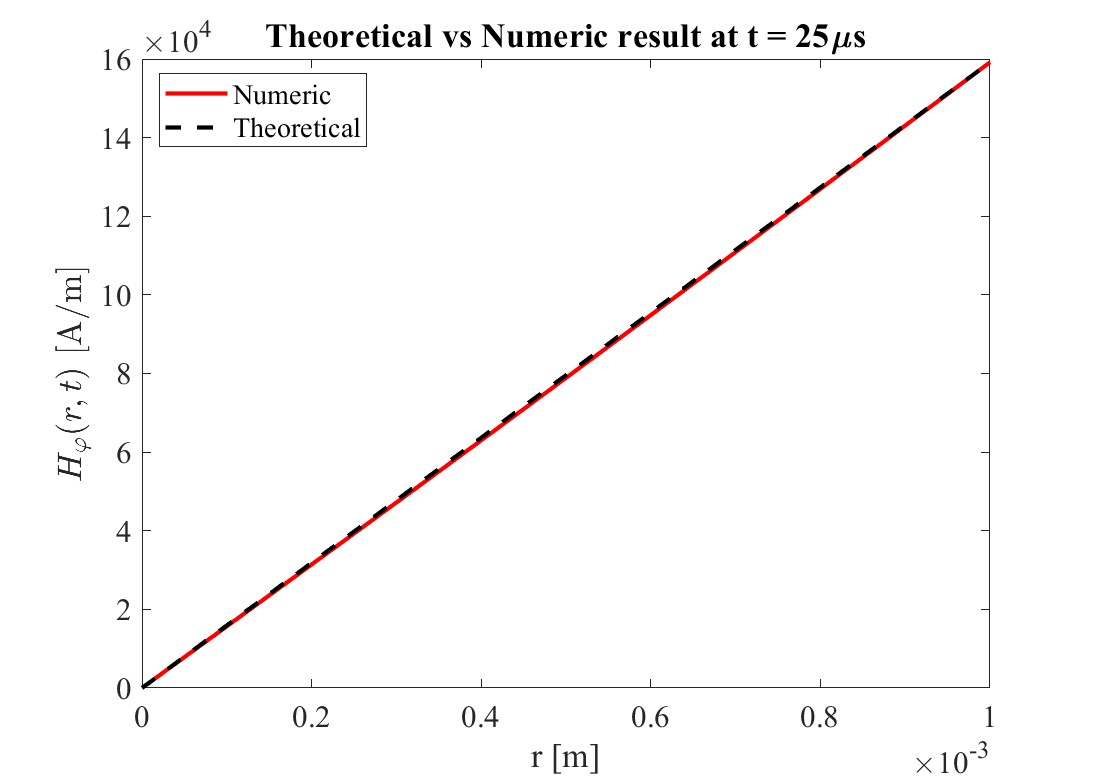
\includegraphics[scale=0.25]{test_plot_figures}
\caption{Comparison of the theory with the numeric result.}
\end{figure}

Note that the resulting curves are identical, as expected. We should also remember that to test the behavior of the current density, we need to integrate the current density over the cross-section surface of the conductor. We will show this during the results.

\subsection{Results}

\subsubsection{DC Current of 1 kA:}

In figure 2, we can see the results for question 1.a.i. and 1.a.ii:
\begin{figure}[ht]
\centering
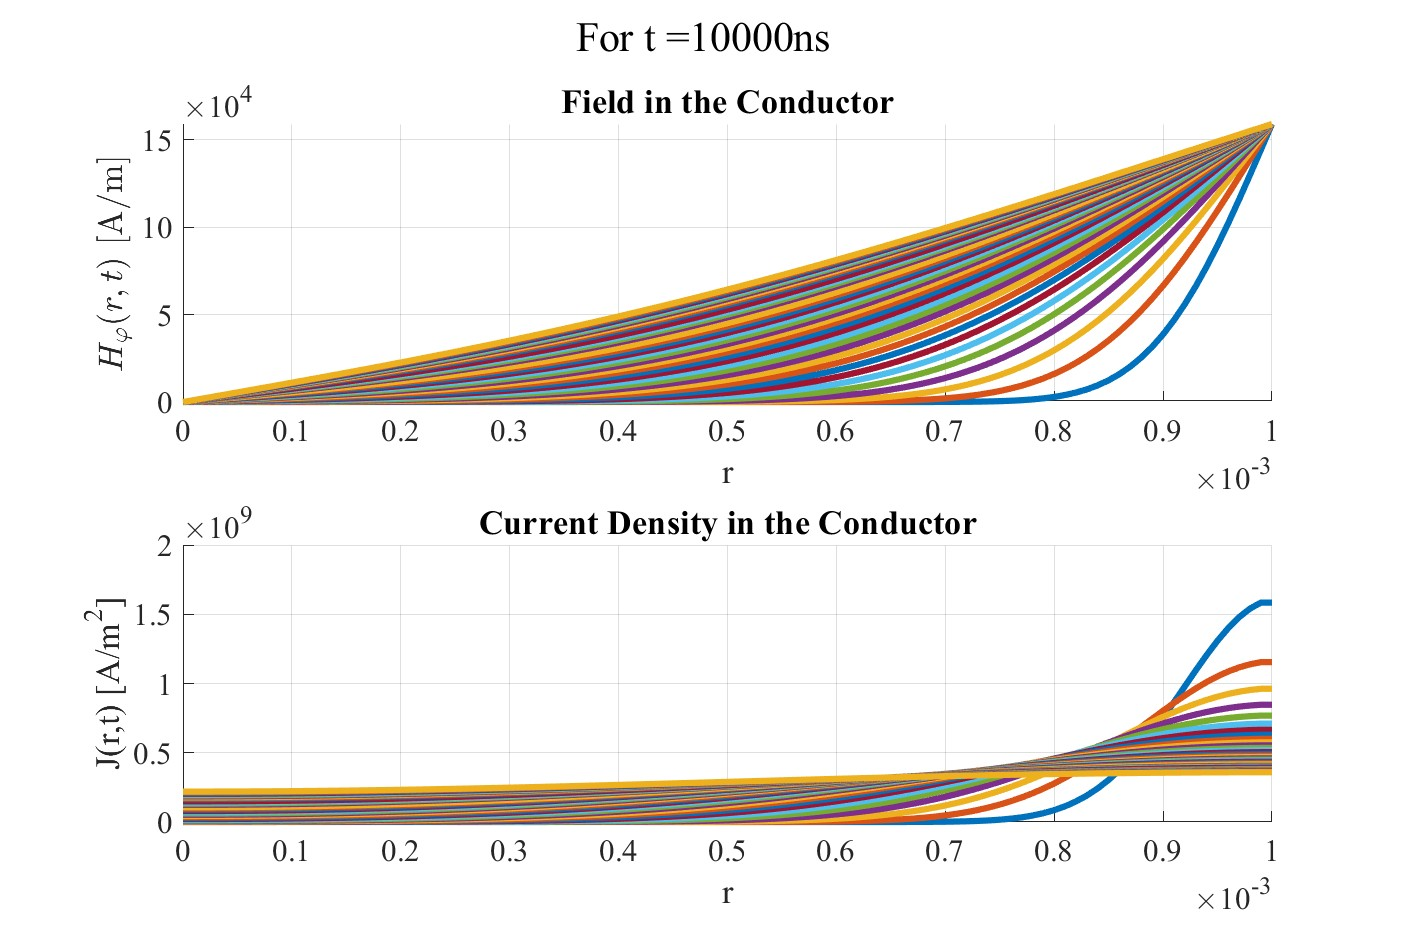
\includegraphics[scale=0.24]{DC_behavior}
\caption{Evolution of the Magnetic Field (top) and the Current Density (Bottom)}
\end{figure}

Initially, the field is very weak in the center of the conductor, and suddenly at around 0.8 mm, it grows exponentially to the boundary condition. The field after some time, behaves more linearly than exponentially, and in the last iteration (for $10 \mu s$, in the top golden line), it looks very similar to the result in Figure 1. Note also that in the bottom plot (for Current Density), the current density is highly concentrated near the boundary of the conductor. However, after some time, it homogenizes across the radius, as expected.

\subsubsection{For AC with f = 100kHz}

\begin{figure}[ht]
\centering
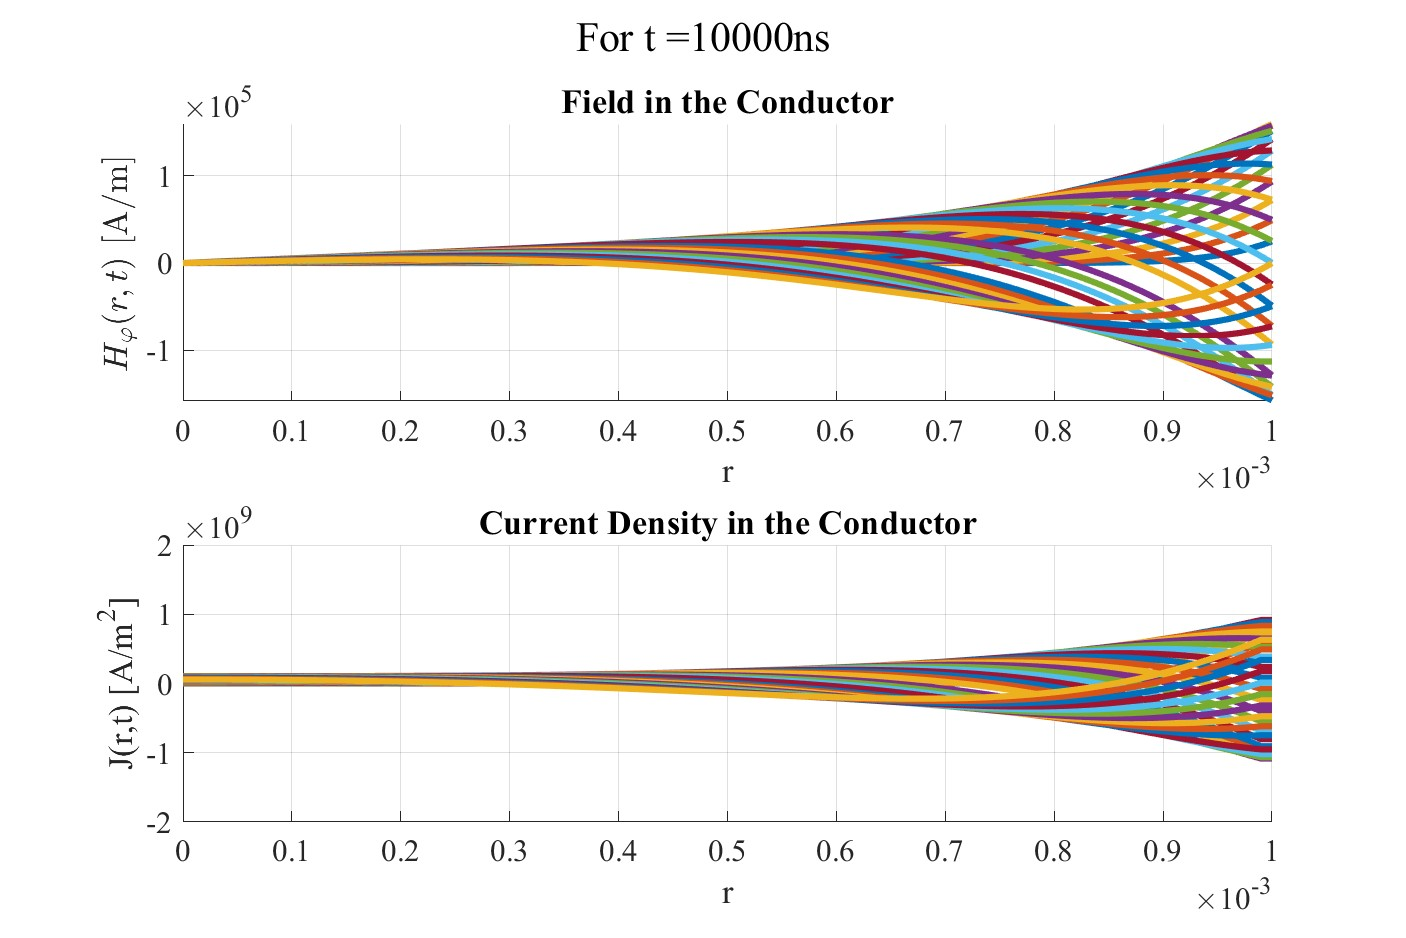
\includegraphics[scale=0.235]{AC_100kHz}
\caption{Evolution of the Magnetic Field (top) and the Current Density (Bottom), for $f = 100kHz$}
\end{figure}

\subsubsection{For AC with f = 1MHz}
\begin{figure}[ht]
\centering
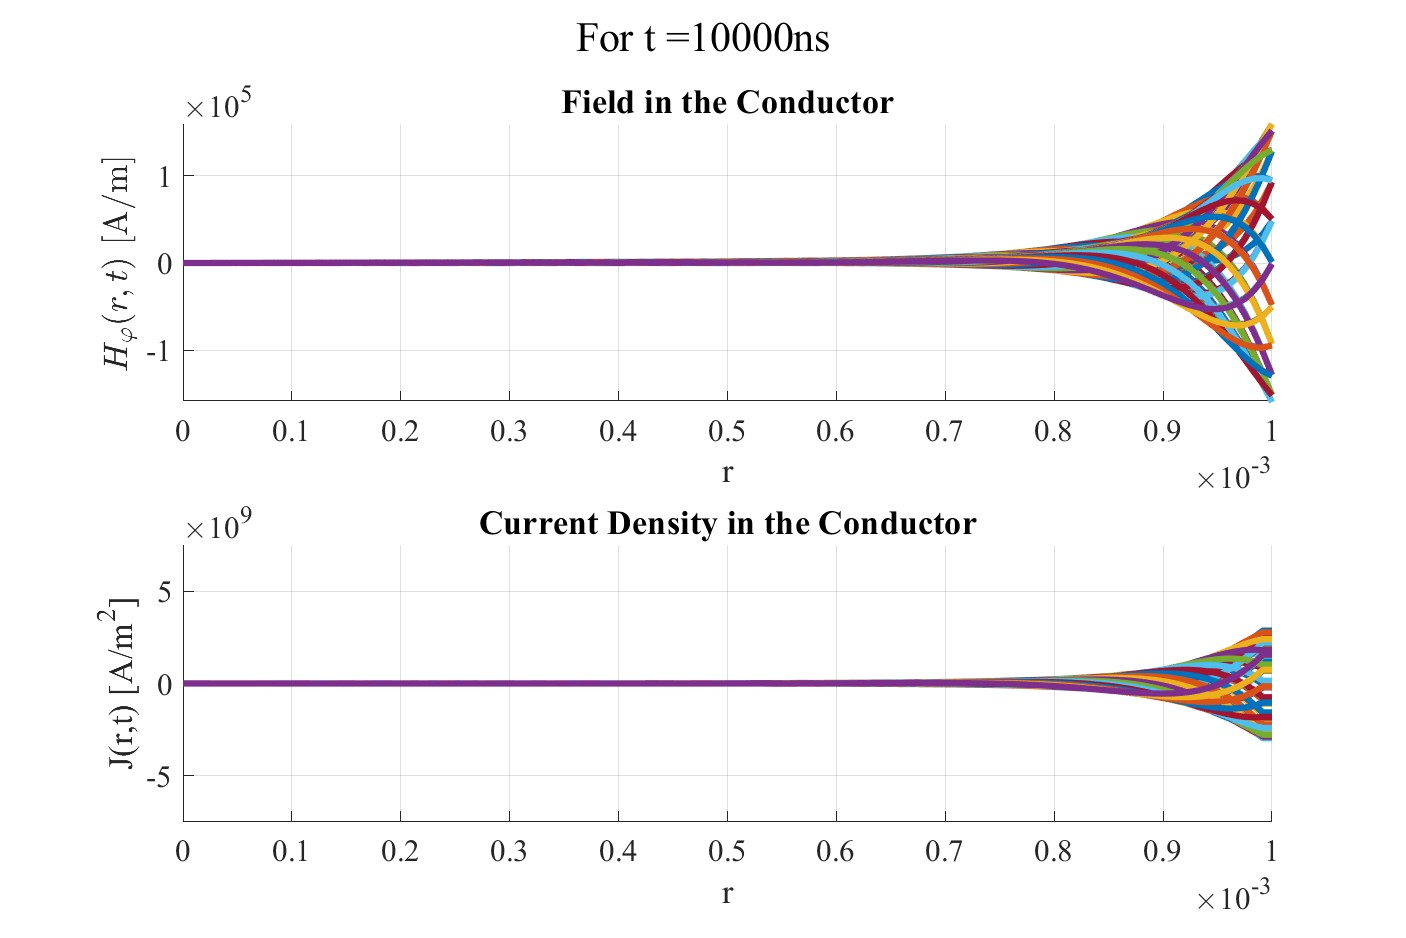
\includegraphics[scale=0.235]{AC_1MHz}
\caption{Evolution of the Magnetic Field (top) and the Current Density (Bottom), for $f = 1MHz$}
\end{figure}
\pagebreak
\subsubsection{For AC with f = 10MHz}

\begin{figure}[ht]
\centering
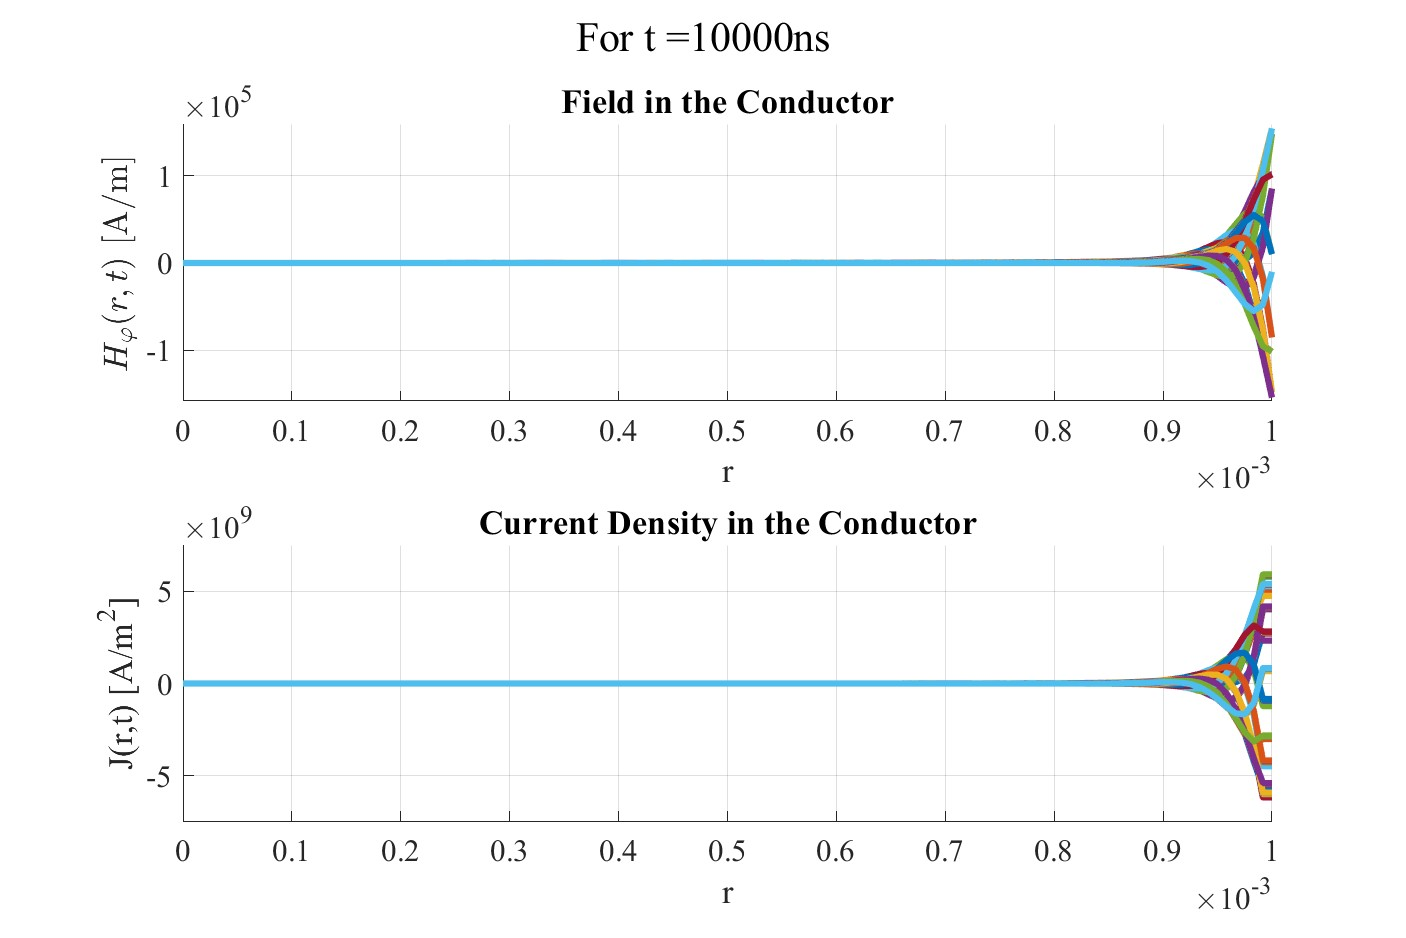
\includegraphics[scale=0.235]{AC_10MHz}
\caption{Evolution of the Magnetic Field (top) and the Current Density (Bottom), for $f = 10MHz$}
\end{figure}

\subsubsection{Analysis for the AC results:}

In figures 3, 4 and 5 we can see the current density and the magnetic field for the three values of frequency. Note that both values are weaker towards the center of the conductor. However, for high values of frequency, the longitude where we can find values of current density and magnetic field, are lower. This is called the \textit{Skin Effect}, where we can see that for higher frequencies, the current is mostly flowing near the surface of the conductor, the "Skin". 

Note also that the values of current density increases for high values of frequency. 

For the 10MHz frequency, we needed to reduce the the $\Delta r$ and $Delta t$ for getting smooth curves. So the integration values are $\Delta r = 1mm/120$, and the $\Delta t = 1 ns$. 

\section{Script Used}

\lstinputlisting[language=Octave]{magnetic_diffusion_polar_coord.m}

\end{document}
